%%%%%%%%%%%%%%%%%%%%%%%%%%%%%%%%%%%%%%%%%%%%%%%%%%%%%%%%%%%%%%%%%%%%%%%%%%%
%
% Plantilla para un artículo en LaTeX en español.
%
%%%%%%%%%%%%%%%%%%%%%%%%%%%%%%%%%%%%%%%%%%%%%%%%%%%%%%%%%%%%%%%%%%%%%%%%%%%

% Qué tipo de documento estamos por comenzar:
\documentclass[a4paper]{article}
% Esto es para que el LaTeX sepa que el texto está en español:
\usepackage[spanish]{babel}
\selectlanguage{spanish}
% Esto es para poder escribir acentos directamente:
\usepackage[utf8]{inputenc}
\usepackage[T1]{fontenc}
%% Asigna un tamaño a la hoja y los márgenes
\usepackage[a4paper,top=3cm,bottom=2cm,left=3cm,right=3cm,marginparwidth=1.75cm]{geometry}

%% Paquetes de la AMS
\usepackage{amsmath, amsthm, amsfonts}
%% Para añadir archivos con extensión pdf, jpg, png or tif
\usepackage{graphicx}
\usepackage[colorinlistoftodos]{todonotes}
\usepackage[colorlinks=true, allcolors=blue]{hyperref}
\usepackage{graphicx}
\usepackage{epstopdf, epsfig}
\usepackage[spanish,es-tabla]{babel}
\usepackage[utf8]{inputenc}
\usepackage{graphicx}
\usepackage{subcaption}

%% Primero escribimos el título
\title{Tarea 2 \\
Cosmología observacional}
\author{Camila Aros Bunster\\
  \small Pontificia Universidad Catolica de Valparaíso\\
  \small arosbunster.cami@gmail.com\\
  \date{}
}

\begin{document}
\maketitle

\begin{abstract}
Se presenta la producción y análisis de un mapa ficticio del CMB, identificando los parámetros cosmológicos que se necesitan para formar un espectro de potencia. Además para la generar estos de espectros angulares de potencias de temperatura, se utilizo  CAMB.
\end{abstract}

\section{\label{sec:introduccion}Introducción}

 El CMB es una tenué radiación de fondo cósmico. Es una fuente importante de datos sobre el universo primitivo porque es la radiación EM más antigua conocida hasta el momento del universo (de la época de la recombinación.
 

CMB es evidencia histórica del origen del Big Bang del universo, es mucho antes de la formación de estrellas, era totalmene denso y caliente. A medida que el universo se expandió, tanto el plasma como la radiación que lo llenaba se empezaron a  enfriar hasta llegar a un momento en que la radiación se desacopla de la materia, y estos foton viajan por el Universo hasta llegar a nosotros, que fue lo que en 1965 casualmente Wilson y Penzias dos radioastrónomos estadounidenses percibieron.

El Espectro de angular de potencia que veremos en este trabajo nos indican muchas cosas sobre el Universo, los primeros peak de este espectro permiten determinar de manera precisa los parámetros que tienen como base el modelo $\lambda$CDM.Los picos impares del espectro corresponden a modos de comprensión del fluido fotón-barión(cuando los fotones caen hacía el potencial). 
En cambio, los picos pares corresponden a modos de rarefacción(la presión de radiación aleja a los fotones del minimo del potencial). Los modos 2 en adelante son modos armonicos del primero, por lo que ocurren en intervalos igual en momentos multipolar"l"

Este trabajo esta organizado de la siguiente manera. Presentamos un resumen sobre las caracteristicas principales del espectro de potencia y en la siguiente sección se explica como se genero un mapa del CMB, en la sección 3 se muestra el proceso inverso para generar un espectro de potencia. Posteriormente en ultima sección presentamos la  conclusión.
.

\section{Generar un mapa del CMB}\label{sec:Generar un mapa del CMB}
 
Para empezar, se nos entrega un espectro de potencia que es el de la Figura 1. 
Teniendo el Espectro Angular de Potencia de Temperatura, podemos generar una aproximación al mapa del CMB.\\

\begin{figure}
\centering
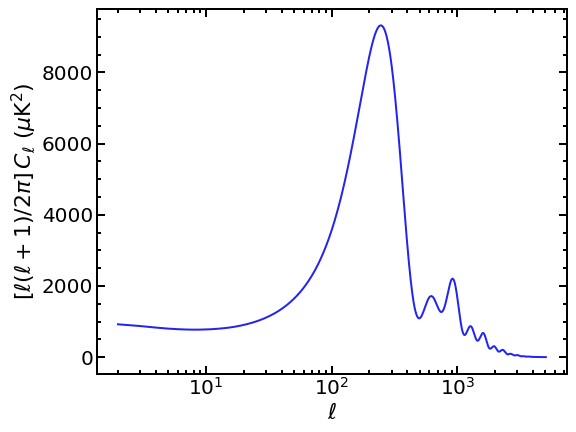
\includegraphics[width=6cm]{D_ell.png}
\centering
\caption{Espectro de potencia angular de las fluctuaciones de temperatura CMB. Se representa $(l(l+1)C_l)/2\pi$  en función de los multipolos "l" (eje inferior).Tenga en cuenta que la escala l cambia de una escala logarítmica para $l\leq 50 $ a una lineal para mayores valores de $l$.}
\end{figure}

Este espectro es generado por fluctuaciones primordiales Gaussianas.Y el mapa observado del CMB esta dado por la siguiente ecuación.

\begin{equation}
    M(\theta_x,\theta_y)=\int dl_x\int dl_y exp[-2i(\vec{l} \cdot \vec{\theta})] \tilde{M}(l_x,l_y)\tilde{G}(l_x,l_y)
\end{equation}

Sabemos que el espectro de potencia esta en función de l y que a la vez esta relacionado con el ángulo que uno observa del cielo $\theta$ (se mide en radianes).Podemos generar un mapa en espacio de fourier de la siguiente manera, 

\begin{equation}
    \tilde{M}(l_x,l_y)=C_l(l)
\end{equation}
\\
Donde l lo podemos expresar en 2 dimensiones.

\begin{equation}
    \tilde{M}(l_x,l_y)=C_l(\sqrt{l_x^2+l_y^2})
\end{equation}
\\
Por el espectro de potencia entregado al inicio de este trabajo, sabemos que l tiene valores que van $0<l<5050$ y por ende $\sqrt{l_x^2+l_y^2}$ tiene como máximo valor 5050. Con esto podemos obtener los $C_l$ respectivo a cada multipolo y así poder obtener $\tilde{M}$ (más detalle ver en el repositorio el Código 1).\\

Una vez que se obtiene $\tilde{M}$ podemos obtener $\tilde{G}$ que es la Transformada de Fourier en 2 dimensiones de un campo gaussiano aleatorio, 
\begin{equation}
    \tilde{G}(l_x,l_y)=\int dl_x \int dl_y exp[-2i(\vec{l} \cdot \vec{\theta})] \eta(\mu ,\sigma )
\end{equation}
\\
Donde $\eta(\mu,\sigma)$ representa al campo gaussiano aleatorio y $\sigma$ determina la amplitud de las fluctuaciones respecto a $C_l$. Para este caso, se tomaron los valores de $(\mu,\sigma)$ como (0,1).\\

Ahora bien, hay que tener en cuenta que se quiere lograr un mapa con una resolución de 0.5 arcmin en una escala de $[10^\circ,10^\circ]$, por lo tanto $10^{\circ}/0.5'\sim 1200 pix$ (todo en radianes) esto nos dice que el mapa del CMB debe ser de(1200,1200).
También hay que fijar $l_{max}$ y $l_{min}$, y para esto hay que tener en consideración la relacion de l con el ángulo en el cielo a través de  $l=2\pi/\theta$, por consiguiente,\\
$l_{max}=2\pi/0.5'=43200$pixeles y para $l_{min}$ hay que tomar $\theta_{max}=\sqrt{(10^{\circ})^2+(10^{\circ})^2}$(en radianes), por lo tanto $l_{min}=2\pi/\theta_{max} \sim 26$ y por último, para obtener un mapa de  1200x1200 nuestro calculos tienen que tener saltos de $43200/1200 =36$.\\

El resultado final del mapa observado del CMB que se puede apreciar en la Figura 2. Este mapa tiene la resolución  que corresponde al tamaño de los pixeles en los mapas entregados por el ACT y SPT (0.5')\\

\begin{figure}
\caption{Mapa del CMB con una resolución de 0.5'}
\centering
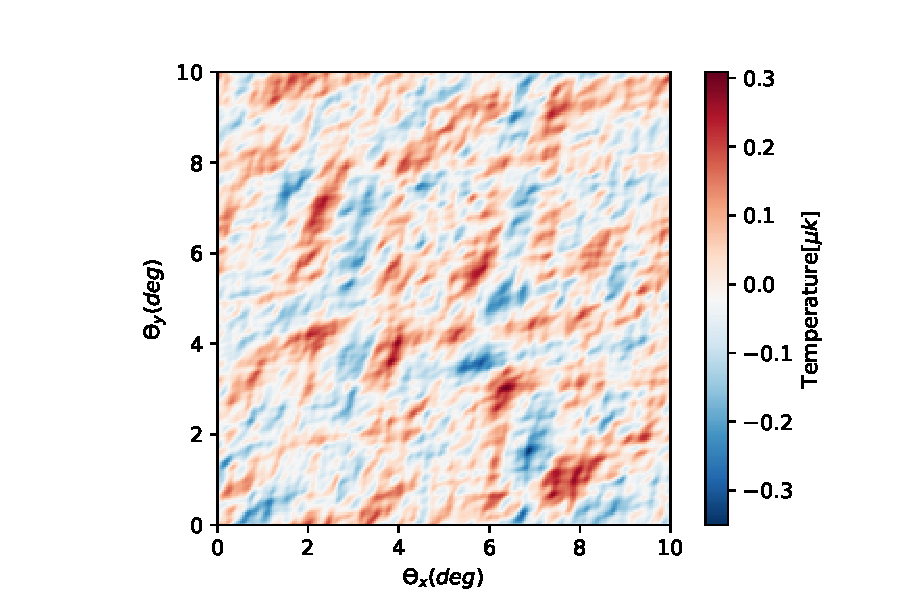
\includegraphics[width=10cm]{CMBfinal.pdf}
\end{figure}

\begin{figure}
\centering
\begin{subfigure}[b]{0.45\linewidth}
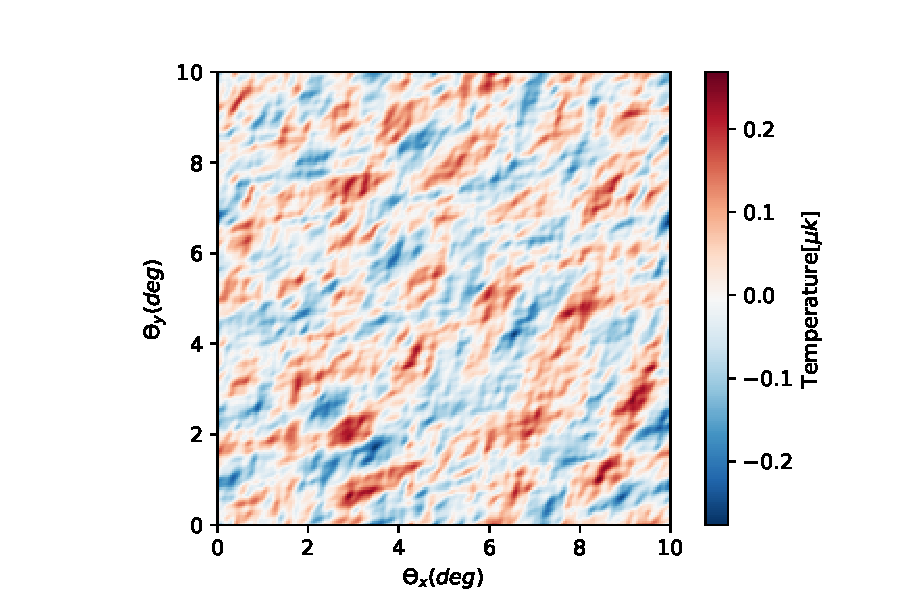
\includegraphics[width=\linewidth]{CMB1ma.pdf}
\caption{Resolución de 1.0'}
\label{fig:CMB1ma}
\end{subfigure}
\begin{subfigure}[b]{0.45\linewidth}
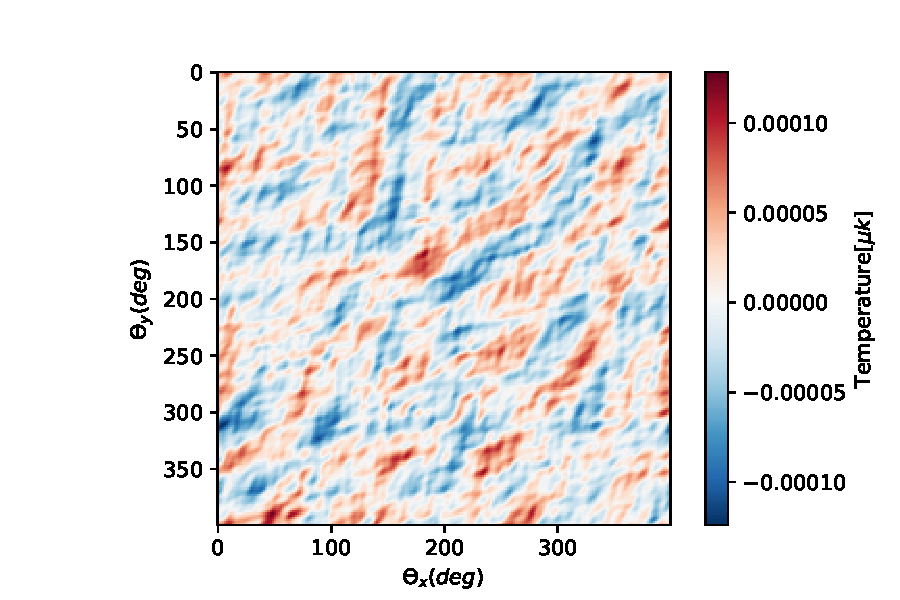
\includegraphics[width=\linewidth]{CMB15ma.pdf}
\caption{Resolución 1.5'}
\label{fig:CMB15ma}
\end{subfigure}
\begin{subfigure}[b]{0.45\linewidth}
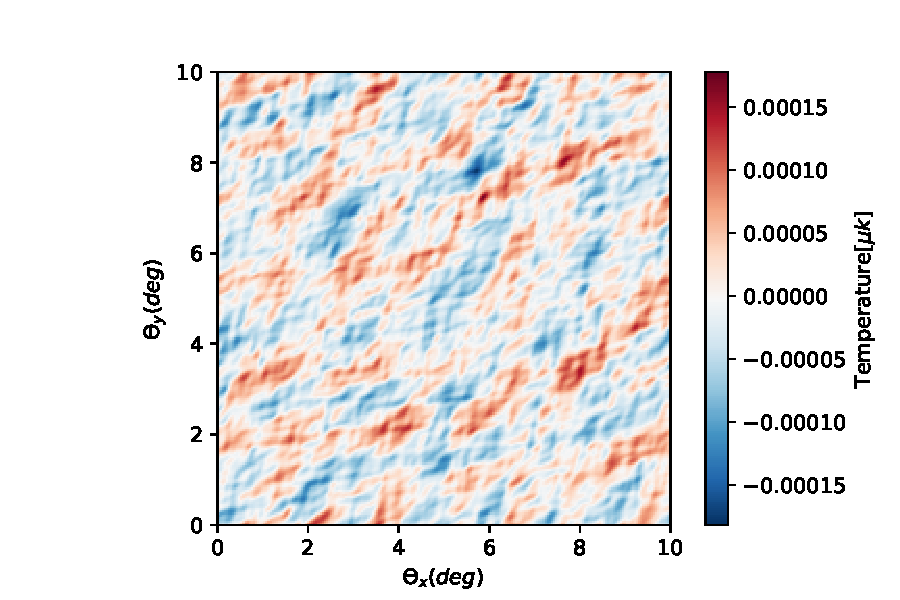
\includegraphics[width=\linewidth]{CMB2ma.pdf}
\caption{Resolución 2.0'}
\label{fig:CMB2ma}
\end{subfigure}
\begin{subfigure}[b]{0.45\linewidth}
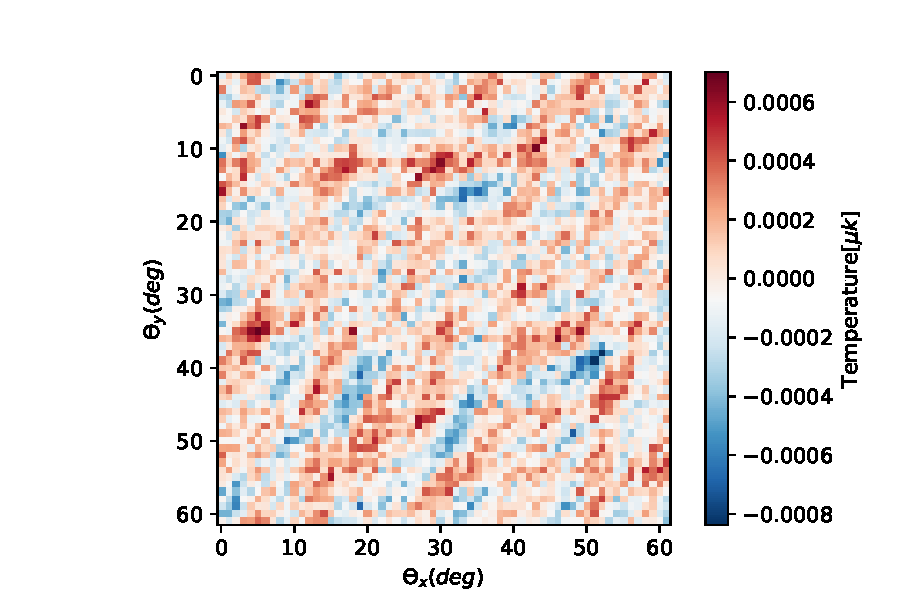
\includegraphics[width=\linewidth]{CMB96ma.pdf}
\caption{Resolución 9.6'}
\label{fig:CMB2ma}
\end{subfigure}
\caption{Mapas del CMB con distintas resoluciones}
\label{fig:westminster}
\end{figure}

En la Figura 3, se observa una comparación de Mapas del CMB con distintas resoluciones. 
En (a) el rango de l era de $26<l<21600$ con saltos de 36 teniendo una matriz de 600x600. 
En (b) se ocupo una resolución de 1.5 arcmin donde el rango de l es  de $26<l<14400$  con saltos de 36, obteniendo una matriz de (400x400).
En la (c) se ocupo una resolución de 2.0 arcmin donde el rango de l es de $ 26<l<10800$ con saltos de 36, obteniendo una matriz de (300x300).
En (d) se ocupo una resolución como el experimento de Planck de 9.6 arcmin donde el rango de l es de $26<l<2249$ con saltos de 36, obtenieneo una matriz de (62x62).\\

Ahora bien, ¿Qué elementos faltaron considerar para tener un mapa realista a esta escala y con esta resolución?


\section{Espectro de potencias}
En esta sección se obtendra el espectro de potencia a partir del Mapa generado en la sección 2

\subsection{Apodización}
¿Por qué se necesita hacer apodización?, la respuesta es muy siemple, si se toma directamente la Transformada de Fourier en 2D del Mapa generado,habría discontinuidad en los bordes, y para evitar este problema apodizamos nuestro mapa.

En que consiste esto, una apodización es una función matemática que tiene valor cero fuera del rango que uno elige,es decir, es una función que hace que el mapa se haga cero a medida que se acerca a los bordes. Este tipo de funciones matemáticas se llaman Window Function.

La función que se eligió fue la función seno (Sine Window) 
\begin{equation}
    W(n)=sin\left ( \frac{n\pi}{N} \right )
\end{equation}

donde N es el numero lineal de pixeles del mapa generado (que en este caso es de 1200) y n son números enteros que van desde 0 hasta N.
Ahora bien, está función es para una dimensión, y  lo necesitamos para  2 dimensiones.
Entonces,
\begin{equation}
    W(n_x,n_y)=sin\left ( \frac{n_x \pi}{N} \right )sin\left ( \frac{n_y\pi}{N} \right )
\end{equation}

Tal que, el mapa apodizado será,
\begin{equation}
   M_{apod}(\theta_x,\theta_y)=M(\theta_x,\theta_y) \circ W(\theta_x,\theta_y)
\end{equation}

donde M es un Producto de Hadamard, y $\circ$ es el operador multiplicativo por elemento. Y el resultado de la apodización lo podemos ver en la Figura 4.

\begin{figure}
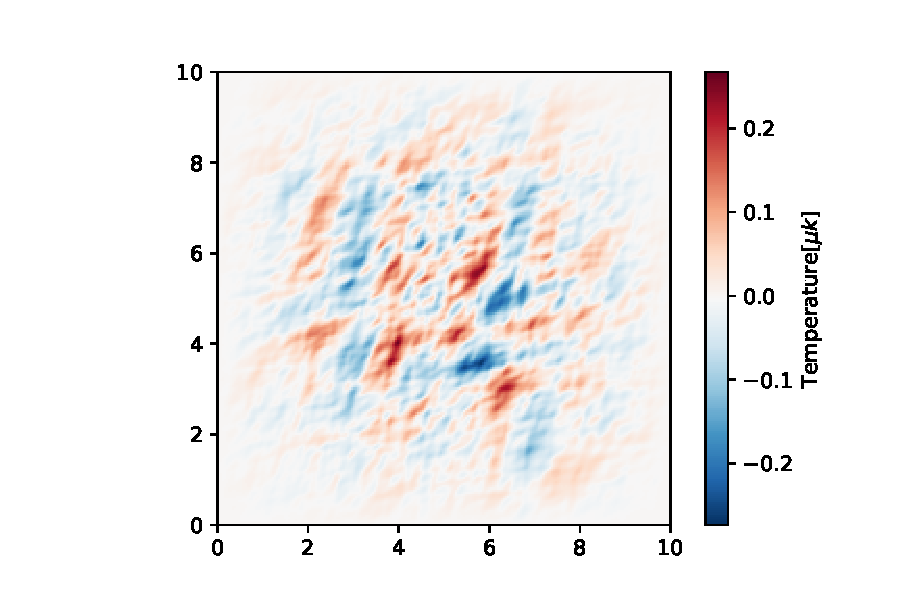
\includegraphics[width=10cm]{CMBapodafinal2.pdf}
\centering
\caption{Apodización del Mapa Generado, es decir, Mapa del CMB que se multiplico por una función seno(Sine Window) para evitar la discontinuidad en los bordes.}
\end{figure}

\subsection{Espectro de potencia}
Como estamos haciendo el proceso inverso de la Sección 2. El espectro de potencia se obtiene tomando la Transformada de Fourier en dos dimensiones del mapa apodizado (que se calculo en la secc.3.1) 
\begin{equation}
    \tilde{M}(l_x,l_y)=FFT(M_{apod}(\theta_x,\theta_y))
\end{equation}

Al calcular $\tilde{M}$ el espectro de potencia se obtiene promediando mapas de anillos con l constante, y en este caso ocupamos un rango de 25, es decir, se tomaban 0<l<25,25<l<50,... y el resultado se eleva al cuadrado .
\begin{equation}
    \left \langle \tilde{M}(l_x,l_y) \right \rangle =C_l\left ( \sqrt{l_x^2+l_y^2} \right )
\end{equation}
 Una vez que se consigue los valores de $C_l$ podemos obtener el espectro de potencia, de la siguiente manera.
 
\begin{equation}
    D_{espectro}=\frac{l(l+1)C_l}{2\pi}
\end{equation}
 
 En la Figura 5, podemos ver el resultado del espectro de potencia,si hacemos una comparación con el espectro de potencia original(Figura 1)vemos que hay una gran diferencia en magnitud, el espectro del mapa generado es 250 veces más grande al original, además  el espectro original aumenta a partir de $l\leq50$, en cambio, el espectro generado aumenta desde el comienzo $l>5$.
 
\begin{figure}
    \centering
    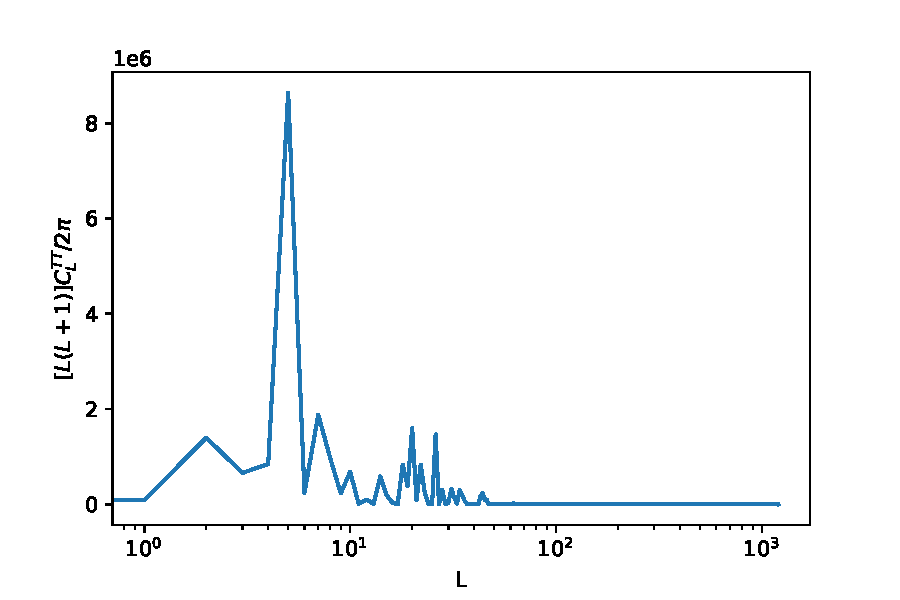
\includegraphics[width=8cm]{espectrodepotencia.pdf}
    \caption{Espectro de potencia del mapa generado del CMB(Sección 1)}
    \label{fig:my_label}
\end{figure}

\subsection{Corrección de sesgos}

Al calcular el espectro de potencia de esta manera(sección 3.2)estamos ignorando algunos errores producto de la apodización y la resolución que le hicimos a nuestro mapa generado.

Para corregir este espectro  y obtener el  espectro de potencia real debemos calcular,
\begin{equation}
    D_l=\frac{(\hat{D_l}-N_l)}{T_l}
\end{equation}

Donde  $T_l$ es la función de transferencia, $N_l$ es el sesgo de ruido,$\hat{D_l}$ es el espectro de potencia que calculamos en la Sec.3.2.
 \subsubsection{Función de transferencia}
 Es una corrección al espectro de potencia generado y depende de la resolución del telescopio y el tamaño del mapa.
 
\subsubsection{Sesgo de ruido}
El sesgo de ruido se obtiene generando mapas que solo contengan ruido, un ejemplo, es $\tilde{G}$ que calculamos en la Sección 2, y el espectro resultante es el sesgo de ruido.

\section{Estimación de parámetros cosmológicos}

En esta sección, identificaremos los parámetros cosmológicos (de manera aproximada) usados para generar el espectro de potencia inicial(Figura 1). \\

Para esta parte, se uso CAMB para generar los espectros de potencia modificando solamente los parámetros $\Omega_c h^2$ y $\Omega_b h^2$\\

\begin{table}[h!]
  \begin{center}
\def~{\hphantom{0}}
  \begin{tabular}{lcccccc}
    $A_s$  & $n_s$   &   $r$ & $H_0(km^{-1}Mpc^{-1})$ & $\sum m_\upsilon (eV)$ & $\Omega_k$ & $\tau$  \\[3pt]
    \hline
    $210^{-9}$ & 0.965 & 0.00 & 67.5 & 0.06 & 0.00 & 0.06\\
\end{tabular}
\caption{Parámetros cosmológicos incorporados en el espectro de potencia.}
\label{tab:kd}
\end{center}
\end{table}
\begin{figure}
    \centering
    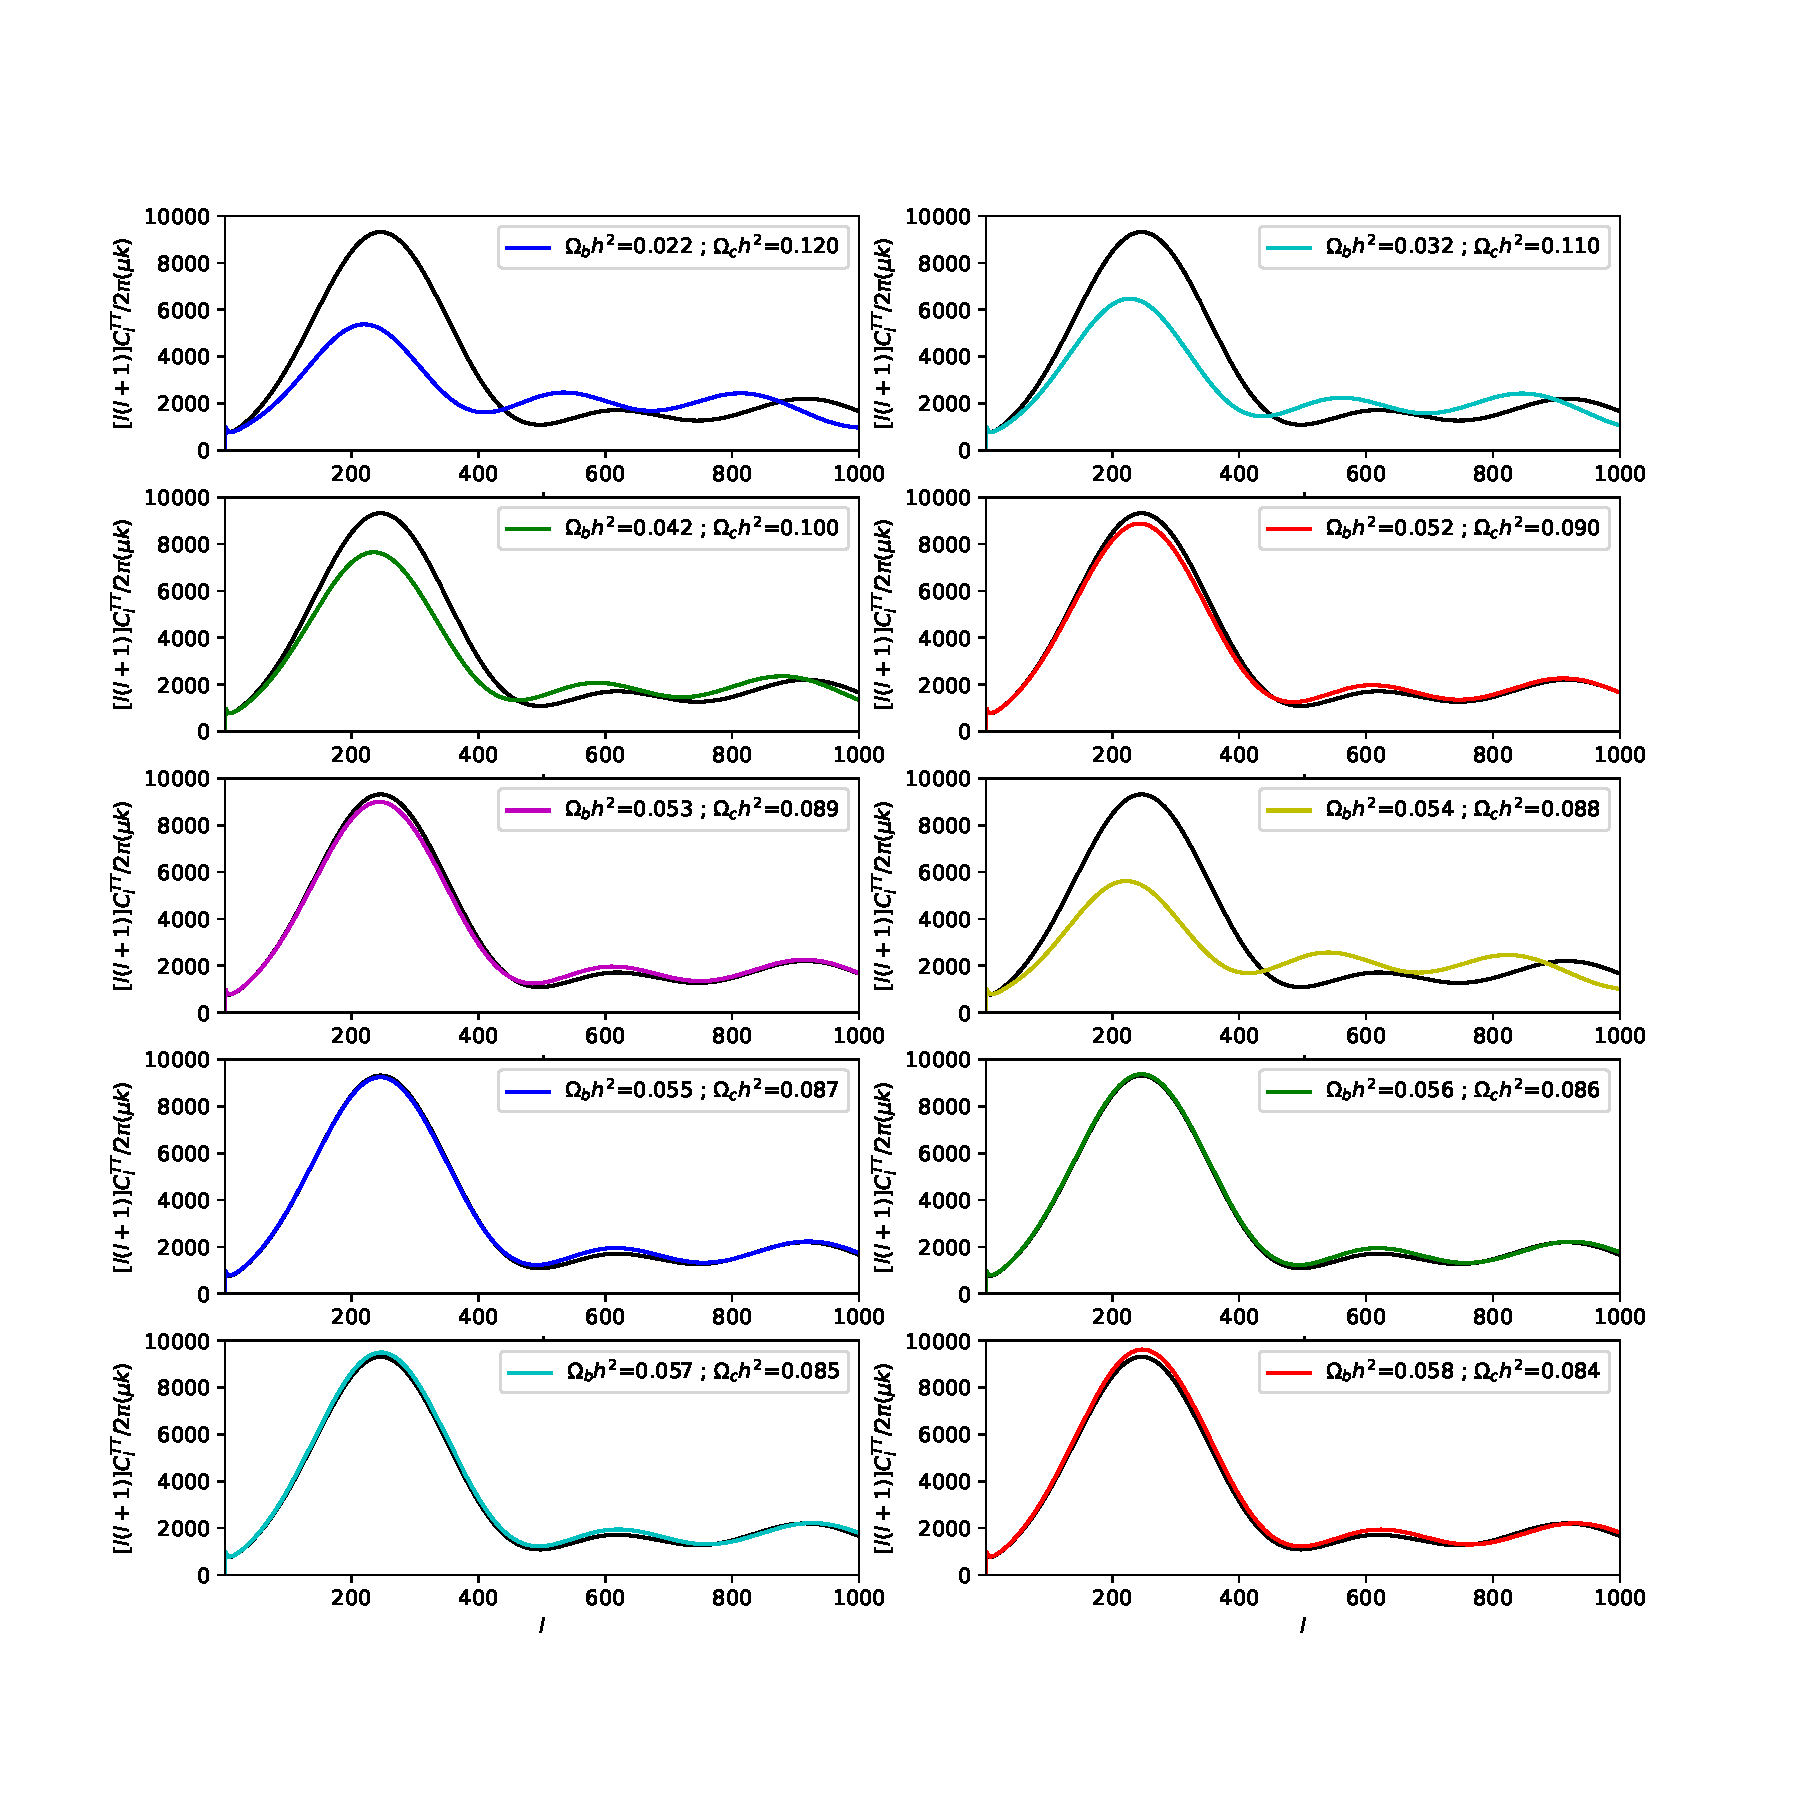
\includegraphics[width=15cm]{comp_param2.pdf}
    \caption{Comparación del espectro original(línea negra) con los espectros generados variando los parámetros $\Omega_c h^2$ $\Omega_b h^2$.  }
    \label{fig:my_label}
\end{figure}

En la tabla 1 se muestran los parametros cosmológicos que se usaron de manera constante, y en la Figura 6 se ve la comparación del espectro original con los espectros generados, podemos ver que los últimos 4 gráficos son los que mejor se ajustan al espectro original.\\

Para que sea más evidente seleccionamos los últimos 3 para ver en mayor detalle, podríamos decir que $0.056\leq \Omega_bh^2\leq 0.058$ y $0.086\leq \Omega_ch^2\leq 0.084$, pero  el mejor valor que se ajusta al espectro de potencia original es de $\Omega_c h^2$=0.056 y $\Omega_b h^2$=0.086.

\begin{figure}
    \centering
    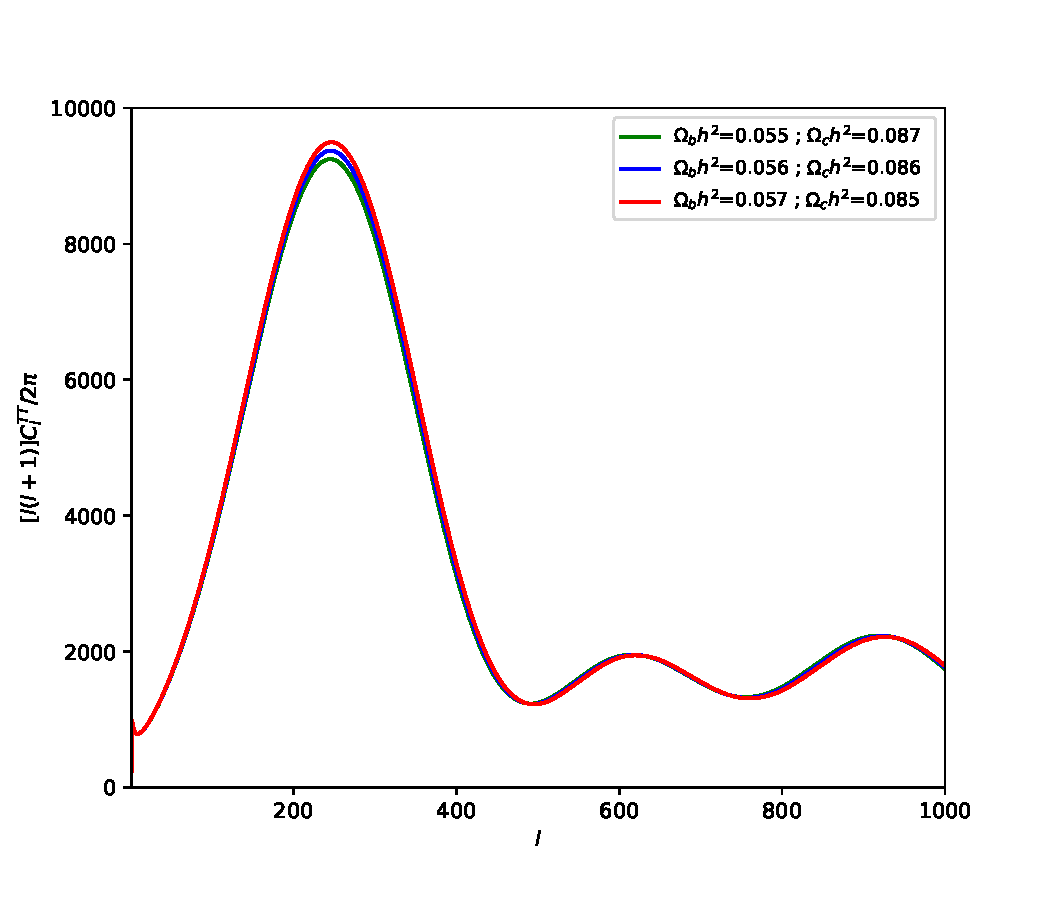
\includegraphics[width=8cm]{mejores_parametros.pdf}
    \caption{Se tomaron los últimos 3 gráficos de la Figura 6, y se hace una comparación con el espectro original y el mejor valor que se ajusta es $\Omega_c h^2$=0.056 y $\Omega_b h^2$=0.086}
    \label{fig:my_label}
\end{figure}

\section{Conclusiones}

En este trabajo se genero un mapa del CMB en base a un espectro de potencias, para luego hacer el proceso inverso y a partir del mapa generar el espectro de potencia. Este último espectro no quedo de la manera correspondiente,una de las posibles razones a este error puede ser un mal planteó al inicio  del código, que por efecto en cadena, arrojaría un mal espectro

En la última parte de este trabajo se analizo el espectro de potencias entregado a un comienzo, y se fue variando los valores de $\Omega_bh^2$ y $\Omega_ch^2$ obteniedo como mejor valor 0.056 y 0.086 respectivamente. 

\section{Referencias}
\bibliographystyle{abbrv}
\bibitem{Louis} \textsc{Thibaut Louis},
\textit{The Atacama Cosmology Telescope: two-season ACTPol spectra and parameters, 2017.}

\bibitem{Henning} \textsc{J.W.Henning },
\textit{Measurements of the Temperature and E-Mode polarization of the CMB from 500 square degrees of SPTPol Data, 2018.}

\bibitem{Das} \textsc{Das },
\textit{The Atacama Cosmology Telescope: Temperature and gravitational lensing power spectrum measurements from three season of data, 2013.}

\bibitem{Dunkley} \textsc{Dunkley },
\textit{The Atacama Cosmology Telescope: Likelihood for small-scale CMB data, 2013.}

\bibitem{Louis }\textsc{Louis },
\textit{Lensing simulation and Power Spectrum Estimation for High Resolution CMB Polarization Maps, 2013}

\bibitem{Naess} \textsc{Naess },
\textit{The Atacama Cosmology Telescope:CMB polarization at 200 <l< 9000,2014.}
\bibliography{sample}

\end{document}
